\section{Brief History of Burgers' Equation}
    
    The simplest fluids (called Newtonian fluids), are described by the well-known Navier-Stokes equations, named after Claude-Louis Navier and George Gabriel Stokes. These are a set of non-linear (PDEs), which are obtained by applying the principles of conservation of mechanics and thermodynamics on a volume of fluid to obtain the so-called integral formulation of the equations. Applying certain considerations, especially those in which the tangential forces have a linear relationship with the velocity gradient (Newton's viscosity law), the differential formulation is obtained which is generally more useful for solving the problems that arise in the mechanics of fluids. For further details about the Navier-Stokes equations see \cite{Acheson2001, Batchelor1967, Landau1987, Currie1974, Temam1984}. \\
    
    Let $v$ be a vector field, Navier-Stokes equations are given as follows
    \begin{equation}
        \left \lbrace \begin{array}{ll}
    	\nabla \cdot v = 0, \\
    	(\rho v)_t + (\nabla \cdot \rho v) v + \nabla p - \mu \nabla^2 v - \rho G = 0.
    	\end{array}  \right .
    	\label{navierstokes}
    \end{equation}
    It is well known that when $\rho$ is considered the density, $p$ the pressure, $v$ the velocity and $\mu$ the viscosity of a fluid, these equations describe the dynamics of an incompressible fluid (free divergence, and $\rho_t = 0$), where $G$ represents the gravitational effects. \\
    
    In contrast to equation (\ref{navierstokes}), this can be investigated in one spatial dimension. Simplification in (\ref{navierstokes}) of the $x$ component of the velocity vector, which we will call $v^x$, gives
    \begin{equation*}
        \rho \frac{\partial v^x}{\partial t} + \rho v^x \frac{\partial v^x}{\partial x} + \rho v^y \frac{\partial v^x}{\partial y} + \rho v^z \frac{\partial v^x}{\partial z} + \frac{\partial p}{\partial x} - \mu \left(\frac{\partial^2 v^x}{\partial x^2} + \frac{\partial^2 v^x}{\partial y^2} + \frac{\partial^2 v^x}{\partial z^2} \right) - \rho G^x = 0.
    \end{equation*}

    \noindent Considering a $1D$ problem with no pressure gradient, the above equation reduces to\\
    \begin{equation}
        \rho \frac{\partial v^x}{\partial t} + \rho v^x \frac{\partial v^x}{\partial x} - \mu \frac{\partial^2 v^x}{\partial x^2} - \rho G^x = 0.
        \label{1.2}
    \end{equation}
    If we use now the traditional variable $v$ rather than $v^x$, take $\alpha$ to be the kinematic viscosity, i.e, $\alpha = \frac{\mu}{\rho}$ and $G \equiv 0$, then the equation (\ref{1.2}) becomes just the viscid Burgers' equation
    \begin{equation}
    \label{Burgers_Equation}
        \frac{\partial v(x, t)}{\partial t} +  \underbrace{v(x, t) \frac{\partial v(x, t)}{\partial x}}_{\textbf{Convection}} - \underbrace{\alpha \frac{\partial^2 v(x, t)}{\partial x^2}}_{\textbf{Diffusion}} = 0.
    \end{equation}

    Some assumptions  are  made,  namely: $\rho =$ constant (density), $\mu =$ constant  (viscosity),  $p=$ constant (pressure). \\
    
    Burgers' equation was introduced in 1915 by Harry Bateman \cite{Bateman1915}, an English mathematician, in his paper along with its corresponding initial condition and boundary values. Later in 1939, Johannes Martinus Burgers \cite{Burgers1939,Burgers1948}, a Dutch physicist, simplified the Navier-Stokes equation (\ref{navierstokes}) by just dropping the pressure term, and in 1948 explained the  mathematical modeling of turbulence with the help of the equation (\ref{Burgers_Equation}). The name of this equation is because Burgers became one of the leading figures in the field of fluid mechanics and, therefore, honors his contributions. \\  
    
    The equation (\ref{Burgers_Equation}) is a partial differential equation nonlinear, where the second term is known as the convective part of the equation and the third as the diffusive part. This equation appears in several areas of applied mathematics, such as fluid mechanics, nonlinear acoustics, gas dynamics, traffic flow, and many others. It is generally considered a toy model, i.e., a tool that is used to understand part of the internal behavior of the general problem.  \\
    
    The formulation given by the equation (\ref{Burgers_Equation}) is called the strong form, i.e., the partial differential equation requires that it be satisfied for each point $x$ in its domain and for each $t$. This formulation can be written as follows
    \begin{equation}
    	\frac{\partial v}{\partial t} + A(v) + F(v) = 0, \hspace{2mm} t > 0,
    	\label{strong}
    \end{equation}
	where $F$ and $A$ are given by
	\begin{equation*}
		A(v) = - \alpha v_{xx}, \hspace{3mm} F(v) = \frac{1}{2} (v^2)_x , \hspace{3mm} x \in I.
	\end{equation*} 
	Multiplying both sides of (\ref{strong}) by $\phi \in X$, for some arbitrary smooth function $\phi$ of compact support, such that the integral of the PDE over the space $I$ is satisfied, we get   
    \begin{equation}
    	\displaystyle \int_{I} \frac{\partial v}{\partial t} \phi dx + \int_{I} A(v) \phi dx + \int_{I} F(v) \phi dx = 0, \hspace{2mm} \forall \phi \in X,\hspace{2mm} \forall t > 0.
    	\label{weak}
    \end{equation}
	The formulation (\ref{weak}) is called the weak form of (\ref{Burgers_Equation}) and $\phi$ are known as the test functions.  If we denote $\langle \cdot, \cdot \rangle$ as the inner product in $X$, then (\ref{weak}) can be written in compact form as follows
    \begin{equation}
    	\left \langle \frac{\partial v}{\partial t} + A(v) + F(v), \phi\right\rangle = 0, \hspace{2mm} \forall \phi \in X, \hspace{2mm} \forall t > 0.	
    	\label{compact_weak}
    \end{equation}
	Note that the two formulations, (\ref{weak}) and (\ref{strong}), are equivalent if the solution is smooth enough, however the weak formulation can adjust less regular solutions than in the strong form. In fact, the solution to (\ref {weak}) is known as the distribution solution of the original equation (\ref{Burgers_Equation}), since it can be shown to satisfy (\ref{Burgers_Equation}) in the sense of distributions. For more details of the above it is recommended to see Schwartz \cite{Schwartz1966}, Lions and Magenes \cite{Lions1972}, Renardy and Rogers \cite{Renardy1993}. \\
	
	Proper use of these formulations allows one to recover the strong form from the weak form, therefore, an appropriate way to design a numerical method is to first choose one of the formulations satisfied by the exact solution, then restrict the choice of test functions to a space of finite dimension, to replace $u$ with the discrete solution $u_N$, and possibly to replace the exact integration with quadrature rules. \\
	
   
    \subsection{Analytical solutions for Burgers' equation.}
    
    When we want to know the precision of an approximation, an alternative is through numerical experiments that can be compared with some other solution considered as a good reference. For this type of tests, the better is to have exact solutions to compare with an approximate one, and fortunately the equation (\ref{Burgers_Equation}) can be solved exactly by Hopf-Cole transformation introduced by Eberhard Hopf \cite{Hopf1950} and Julian David Cole \cite{Cole1951} independently to convert the Burgers' equation into a linear parabolic equation and solve it exactly for any initial condition. \\
  
   	\noindent Now consider the problem of initial value for the equation (\ref{Burgers_Equation}) as follows
    \begin{equation}
        \left \lbrace \begin{array}{ll}
    	u_t + u u_x = \alpha u_{xx} & x \in \mathbb{R}, \hspace{2mm} t > 0, \hspace{2mm} \alpha > 0 \\
    	u (x, 0) = u_0 (x)  & x \in \mathbb{R},
    	\end{array}  \right .
    	\label{IVP}
    \end{equation}
	Hence, the transformation known as the Cole-Hopf transformation is given by
    \begin{equation}
        u = -2 \alpha \frac{\varphi_x}{\varphi}
        \label{Hopf_tranform}
    \end{equation}
    Operating (\ref{Hopf_tranform}) into each term of (\ref{IVP}) we find that
    \begin{equation*}
        u_t = \frac{2 \alpha (\varphi_t \varphi_x - \varphi \varphi_{x t})}{\varphi^2} \hspace{2mm} , \hspace{2mm} u u_x = \frac{4 \alpha^2 \varphi_x (\varphi \varphi_{xx} - \varphi^2_x)}{\varphi^3},
    \end{equation*}
    and 
    \begin{equation*}
        \alpha u_{xx} = - \frac{2 \alpha^2 (2 \varphi_x^3 - 3 \varphi \varphi_{xx} \varphi_x + \varphi^2 \varphi_{xxx})}{\varphi^3}.
    \end{equation*}
    Substituting these expressions into (\ref{IVP}),
    \begin{align*}
        \frac{2 \alpha (-\varphi \varphi_{x t} +  \varphi_x ( \varphi_t - \alpha \varphi_{xx}) + \alpha \varphi \varphi_{xxx})}{\varphi^2} = 0, 
    \end{align*}
	so we have the following,
	\begin{align*}    
        - \varphi \varphi_{x t} + \varphi_x (\varphi_t - \alpha \varphi_{xx}) + \alpha \varphi \varphi_{xxx} = 0 &\Longleftrightarrow \varphi_x (\varphi_t - \alpha \varphi_{xx}) = \varphi (\varphi_{x t} - \alpha \varphi_{xxx}) \\
        &\Longleftrightarrow \varphi_x (\varphi_t - \alpha \varphi_{xx}) =  \varphi (\varphi_t - \alpha \varphi_{xx})_x.
    \end{align*}
    Therefore, if $\varphi$ solves the equation $\varphi_t - \alpha \varphi_{xx} = 0$, $x \in \mathbb{R}$, then $u(x, t)$ given by the transformation (\ref{Hopf_tranform}) solves the Burgers equation.\\
    
    \noindent To completely transform the problem (\ref{IVP}) we still have to work with the initial condition function. To do this, note that (\ref{Hopf_tranform}) can be written as
    \begin{equation}
        u = -2 \alpha (\log \varphi)_x,
        \label{Hopf2}
    \end{equation}
    
    \noindent hence, we get
    \begin{equation*}
        \varphi (x, t) = \displaystyle e^{- \int \frac{u(x, t)}{2 \alpha} dx}.
    \end{equation*}
    It is clear from (\ref{Hopf2}) that multiplying $\varphi$ by a constant does not affect $u$, so we can write the last equation as
    \begin{equation}
        \varphi (x, t) = \displaystyle e^{- \int_{0}^{x} \frac{u(y, t)}{2 \alpha} dy}.
        \label{phi}
    \end{equation}
    The initial condition on (\ref{IVP}) must be transformed by using (\ref{Hopf2}) to get
    \begin{equation*}
        \varphi (x, 0) = \varphi_0 (x) = \displaystyle e^{- \int_{0}^{x} \frac{u_0 (y)}{2 \alpha} dy}.
    \end{equation*}
    In summary, we have reduced the problem (\ref{IVP}) to this one
    \begin{equation}
        \left \lbrace \begin{array}{ll}
    	\varphi_t - \alpha \varphi_{xx} = 0,  & x \in \mathbb{R}, \hspace{2mm} t > 0, \hspace{2mm} \alpha > 0, \\
    	\varphi (x, 0) = \varphi_0 (x) = \displaystyle e^{- \int_{0}^{x} \frac{u_0 (y)}{2 \alpha} dy}, & x \in \mathbb{R}.
    	\end{array}  \right .
    \label{heat}
    \end{equation}
    \paragraph{Parabolic Equation.} The general solution of the initial value problem for the equation (\ref{heat}) is well known and can be handled by a variety of methods. An interesting method related to spectral methods is the following: one can take the Fourier transform with respect to $x$ for both the equation and the initial condition $\varphi_0 (x)$ to obtain a first-order (ODE) as follows
    \begin{equation*}
        \left \lbrace \begin{array}{ll}
    	\hat{\varphi}_t = \xi^2 \alpha \hat{\varphi},  & \xi \in \mathbb{R}, \hspace{2mm} t > 0, \hspace{2mm} \alpha > 0, \\
    	\hat{\varphi} (\xi, 0) = \hat{\varphi}_0 (\xi), & \xi \in \mathbb{R},
    	\end{array}  \right .
    \end{equation*}
    where $\hat{\varphi} (\xi, t) = \displaystyle \int_{-\infty}^{\infty} \varphi (x, t) e^{i \xi x} dx $. \\
    
    \noindent Then the solution for this problem is
    \begin{equation*}
         \hat{\varphi} (\xi, t) =  \hat{\varphi}_0 (\xi) e^{ \xi^2 \alpha t}.
    \end{equation*}
    
    \noindent To recover $\varphi (x, t)$ we have to use the inverse Fourier transformation $F^{-1}$ , namely,
    \begin{equation*}
        \varphi (x, t) = F^{-1} (\hat{\varphi} (\xi, t)) = F^{-1} (\hat{\varphi}_0 e^{\xi^2 \alpha t}) = \varphi_0 (x) \ast F^{-1} (e^{\xi^2 \alpha t}),
    \end{equation*}
    where $\ast$ denotes the convolution product.\\
    
    \noindent On the other hand
    \begin{equation*}
        F^{-1} (e^{\xi^2 \alpha t}) = \frac{1}{2 \sqrt{\pi \alpha t}} e^{- \frac{x^2}{4 \alpha t}},
    \end{equation*}
    so the initial value problem (\ref{heat}) has the analytic solution
    \begin{equation*}
        \varphi (x, t) = \frac{1}{2 \sqrt{\pi \alpha t}} \displaystyle \int_{-\infty}^{\infty} \varphi_0 (\xi) e^{- \frac{(x - \xi)^2}{4 \alpha t}} d\xi.
    \end{equation*}
    Finally, from (\ref{Hopf_tranform}), we obtain the analytic solution for the problem (\ref{IVP})
    \begin{equation}
    \label{Exact_Solution}
        u (x, t) =  \displaystyle \frac{\int_{-\infty}^{\infty} \frac{x - \xi}{t} \varphi_0 (\xi) e^{- \frac{(x - \xi)^2}{4 \alpha t}} d\xi}{\int_{-\infty}^{\infty} \varphi_0 (\xi) e^{- \frac{(x - \xi)^2}{4 \alpha t}} d\xi}. 
    \end{equation}
    
    However, the previous solution cannot always be calculated explicitly and we must implement some numerical integration method very efficiently to obtain a good approximation.
    
    \begin{figure}[H]
    	\centering
    	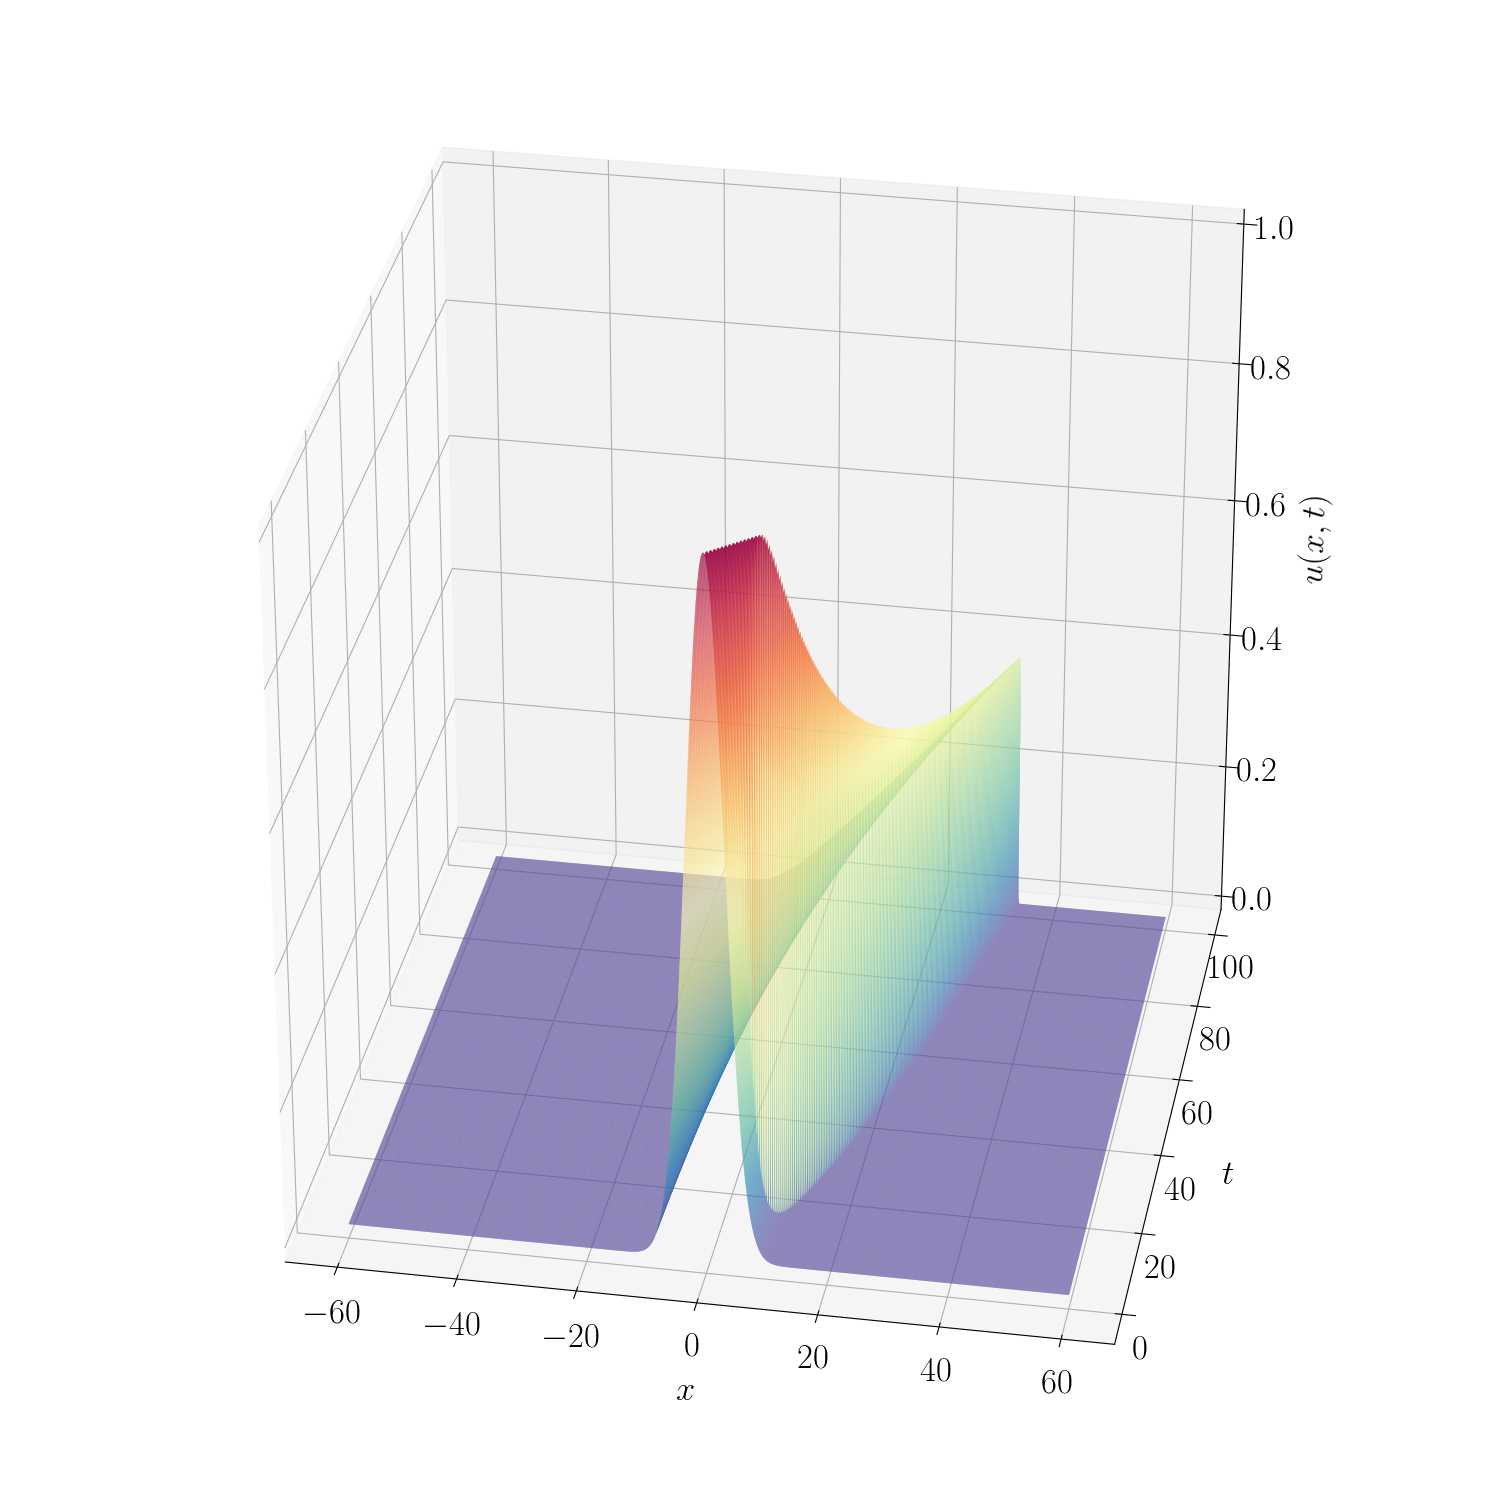
\includegraphics[width=11cm]{introduction/figures/Exact_Solution_alpha=001.png}
    	\caption{Exact solution for (\ref{IVP}) with initial condition $u_0 (x) = e^{-0.05x^2}$ using the equation (\ref{Exact_Solution}) for $x \in [-60, 60]$, $t \in [0, 100]$, and $\alpha = 0.01$.}
    	\label{Exact_Solution_alpha=0.01}
    \end{figure}